\documentclass[12pt]{article}

\usepackage{amssymb,amsmath,amsthm}
\usepackage{graphicx} % Package for including figures
\graphicspath{ {..} }


\begin{document}

\title{HW3: Analysis of Numerical Integration Methods \\ CS471}
\author{Nicholas Livingstone}
\date{\today}
\maketitle

\begin{abstract}
Integration is a critical aspect of many domains of science. Integrating a function by hand can produce exact results,
however this is not always possible and an approximation must be used instead. Different forms of approximation can
have different degrees of accuracy for different functions. In this report, we will analyze two different approaches
to approximating an integral in Fortran: the Composite Trapezoid Rule and Gauss Quadtrature. We will show that both of these methods have 
their advantages and can be more efficient than the other depending on the function being integrated. 

\end{abstract}

\section{Introduction}

In this report, two methods, Composite Trapezoid Rule and Gauss-Legendre Quadrature, will be used to approximate the integral:
\[I =  \int_{-1}^1 e^{\cos{(k x)}} dx\]
for \(k = \pi, \pi^2\). The two methods will be introduced below and then the error of each approach on each function
will be analyzed. 


\subsection{Approximation Methods}
\subsubsection{Composite Trapezoid Rule}
The Trapezoidal Rule is a Newton-Cotes approach to approximating an integral. Newton-Cotes forms of approximations
work by integrating a low-degree function which approximates the original function via interpolation. The
interpolated points of the original function result in the shape of a Trapezoid, producing the name
\emph{Trapezoid Rule}. The composite form of the Trapezoid Rule, which is used in this report, uses the same
idea, but the interval is split into \(n\) sub-intervals. The integral of each sub-interval is then approximated
using the Trapezoid Rule. The Rule is defined as the following: \\


\textbf{Composite Trapezoid Rule Formula}
\[\int_a^b f(x)dx\approx h\left(\frac{f(x_0) + f(x_n)}{2}\right) + \sum_{i = 1}^{n-1} f(x_i)\]

Where \(h\) is defined as \(h = \frac{b-a}{n}\)

\subsubsection{Gauss Quadrature}
Gauss Quadrature works by taking advantage of orthogonal functions and improves on the idea of sub-intervals
characteristic of Newton-Cotes approximation methods. As discussed for the trapzedoial method, a set of 
evenly spaced points is chosen based on \(n\) points. Wtih Gauss Quadrature however, the points are no longer
evenly spaced and a different weight is applied to each area of approximation. This idea is evident in forms
of adaptive quadrature and benificial as it limits the number of operations necessary to integrate certain areas
of the function. For example, say we had a function \(f\) that oscillated greatly from 
-1 to 0, where as from 0 to 1 the function was generally smooth. If we were to use the trapzeoidal method to 
the integral, a large \(n\) would likely have to be chosen to produce an accrate result. The benefits of using
a large number of subintervals would be lost on the interval from 0 to 1, as a just a few would likely be able to
produce a fairly accurate result. Gauss Quadrrature uses this idea in conjunction with orthogonal functions to produce
accurate approximations of integrals for complex equations. Because orthogonal functions are by definition linearly
independent, they can exactly approximate a function of at most \(2n-1\). Any set of orthogonal functions can be chosen,
however for this specific case where the function will be integrated over [-1,1], we shall use the Legendre polynomials,
as they are orthogonal within that interval. When using these specific formulas, the method is called \emph{Gauss-Legendre 
Quadrature}. Each sub-interval approximation is adjusted using
weights \(w_i\) calcluated for each relative \(x_i\) and improves the accuracy of the approximation. Using these exact
function approximations with differently sized and weighted sub-intervals produces a custom fit approximation of the \
integral.\\

\textbf{Gauss Quadrature Formula}
\[\int_{-1}^1 f(z) w(z) dz\approx \sum_{i = 0}^{n} w_i f(z_i)\]

\section{Code-Design}
The code for this report was split into multiple parts. Each method is contained in its own
Fortran file. Both files will loop through the program twice to complete the approximation
for both instances of \(k\). For each loop the program will run for \(n = [1,5000]\). In practice,
this is poor form, but this was elected for the sake of demonstration. The absolute error is calculated
by finding the absolute value of the difference between the previous iteration and the current.
After each loop, the prior approximation is saved for this. This means that the first error should not be
accounted for as a legitimate error. The error is calculated 
for each approximation relative to n and exported to a seperate data file for later
processing in a comma delimmited format. A python script which utilizes the matplotlib library will
then process the files and graph them, which is seen in Figure \ref{fig:graph}. 

\subsubsection{Trapezoidal Rule Implementation}
The Trapezoid Rule is implemented by first calculating the value of \(h\) relative to
\(n\). Then the sum of all \(x_i\)'s is calculated using a do loop. The sum is added
to the remaining terms of the Trapezoid Rule formula to produce the
approximation. The code for this method can be found in Section \ref{trap_code} as
\emph{trapezoidal.f90}.

\subsubsection{Gauss-Legendre Implementation}
The Gauss-Legendre form of approximation is implemented by first allocating space for the
values of \(w_i, w_i,\) and \(f(x_i)\). Then the nodes and weights of the Legendre Polynomials
are found using \emph{lglnodes.f90} (Section \ref{lgl_code}). The program then loops through
the product of each weight and integral approximation and add them to the total approximation.
The error is then calculated and saved. The code for this method can be found in Section \ref{gauss_code} as
\emph{gq.f90}.


\section{Analysis}

\begin{figure}
  \centering
  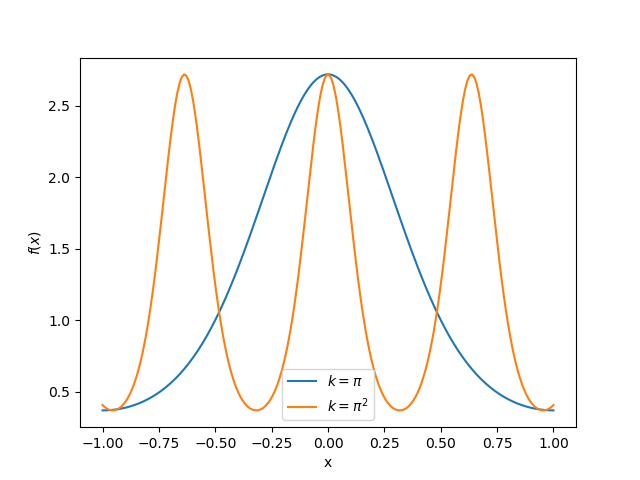
\includegraphics{../figures/functions_plot.png}
  \caption{\(f(x) = e^{\cos{(k x)}}\)}
  \label{fig:function_plot}
\end{figure}

\begin{figure}
  \centering
  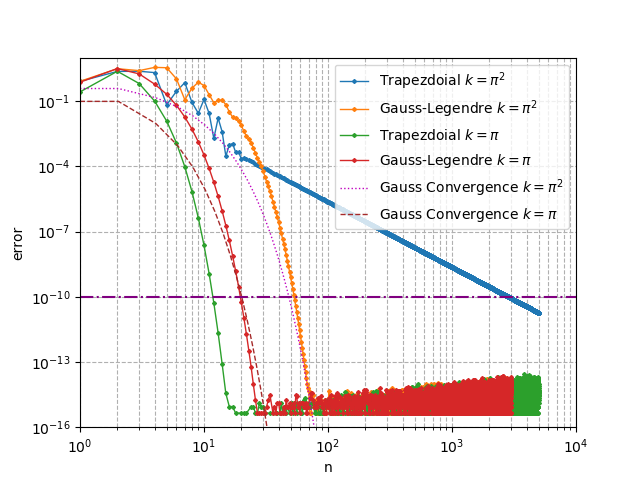
\includegraphics{../figures/graph}
  \caption{Error of Different Integral Approximations}
  \label{fig:graph}
\end{figure}

We can determine the efficiency of both methods by comparing \(n\) to the absolute error. 
It is evident from Figure \ref{fig:graph} that each method is better for different values of \(k\).

\subsection{Why \(k=\pi\) is especially accurate when using the Trapezoid Rule}
The trapezoidal method is clearly more efficient for \(k = \pi\) and in fact faster than Gaussian-Legendre
which can be surprising as Gauss Quadrature is generally considered more accurate. \(n = 12\) is the minimum
value needed to produce an error \(<10^{-10}\) where are as Gauss requires \(n > 20\). From the graph, it can
also be concluded that the Trapezoidal method is second order accurate in this case. This can be seen as the error decreases
by roughly a half when n is doubled for \(k=\pi\). We can additionally see that \(k=\pi\) is a special case
in terms of the efficiency of the Trapezoid rule. It is much more efficient than for \(k=\pi^2\)
because it's a periodically smooth function on [-1,1] (Figure \ref{fig:function_plot}). This allows its integral to be well represented
by a sum. \(k=\pi^2\) is \emph{not} periodally smooth on [-1, 1] which results in the poor accuracy when running
the Trapezoid Rule on this form of the function. 

\subsection{\(k=\pi^2\) and the general efficiency of Gauss Quadrature}
Gauss-Legendre Quadrature is favored in the case of \(k=\pi^2\), but not for the Trapezoid Rule. The graph demonstrates
that generally, Gauss Quadrature will have a consistently more accurate approximation on average, save for the special
case of \(k=PI\). From the graph, we can see that the method exhibits spectral convergance of the form \(\varepsilon(n) \sim C^{-\alpha n}\), 
where \(C\) and \(\alpha\) are constants. By setting \(C=1.1\) and \(\alpha=12, 5\) for \(k=\pi, \pi^2\)
respectively, we can produce a loose approximation of the error curve. These curves can be seen in Figure \ref{fig:graph}

\subsection{Note on larger values of \(n\)}
Additionally, it can be seen on Figure \ref{fig:graph} that once the approximations almost hit \(10^{-10}\) digits
of accuracy, increasing the value of n actually begins to increase the size of the error. This is likely due not to the
methods themselves, but rather the limiations of the computer. Since floating point values generally contain almost 16 digits
of accuracy on 32-bit systems, the computer is likely experiencing some underflow and rounding issues that become
apparent in our graph. 

\section{Conclusion}
In this report, we experimented with two different forms of Numerical Integration,
Trapezoid Rule and Gauss-Legendre Quadrature, and analyzed their accuracy. From the data collected, we determined that
both methods are advantageous depending on the context. This signifies that, when selecting any form of Numerical Analysis,
it's crucial to understand the functions involved and the context, as to select the best approach when completing an
approximation. 

\section{Code}

\subsection{Trapezoid Rule}\label{trap_code}
\subsubsection{trapezoidal.f90}
This file calculates the integral using the Trapezoid Rule for both instances of k and exports the
data to a file. 
\begin{verbatim}
  program trapezoidal
  ! Variables
  implicit none
  double precision :: abs_err = 1D0, sum = 0, xi, approx, prev_approx = 1d0
  double precision, parameter :: X_L = -1d0, X_R = 1d0, max_err = 10D-16
  double precision, parameter :: PI = acos(-1.d0) ! Constant PI 
  double precision, parameter, dimension(2) :: k = (/PI, PI**2/) ! array of k parameters
  real(kind = 8) :: h
  integer :: n = 1, i, j

  ! File Variables
  character(len=10) :: file_id
  character(len=50) :: file_name
  

  do j = 1,2
      ! Setup file-name & open based on which k is being tested
      ! Taken from: https://stackoverflow.com/q/22694626
      write(file_id, '(i10)') j
      file_name = '../../data/trap_data' // trim(adjustl(file_id)) // '.txt'
      open(j, file = trim(file_name))
      
      ! Loop over different values of x
      do while (n < 5000)

          ! Complete Trapezoidal approximation 

          h = (X_R - X_L)/n

          ! Calculate summation term
          do i = 1, (n - 1)
              xi = X_L + (i * h)
              sum = sum + f_x(xi, k(j))
          end do

          ! Calculate integral approximation using Composite Trapezoidal Rule formula
          approx = h * ((f_x(X_L, k(j)) + f_x(X_L + n * h, k(j)))/2 + sum)

          ! Calculate Error
          abs_err = abs(prev_approx - approx)
          
          ! Write Data to file
          write(j, "(i6, a, ES12.6, a, ES17.11)") n, ",", abs_err, ",", approx

          ! Clean up for next iteration
          n = n + 1 ! Iterate n for the next loop 
          sum = 0d0 ! Reset sum to zero
          prev_approx = approx
      end do
      
      close(j)        !close file
      abs_err = 1d0   !reset error
      n = 1           ! reset n
      prev_approx = 0  ! reset previous error
  end do

  
  contains
      include '../functions.f90'

end program trapezoidal
\end{verbatim}

\subsection{Gauss-Legendre Quadrature}
\subsubsection{gq.f90} \label{gauss_code}
This file coputes the integral approximation of the function using
Gauss-Legendre Quadrature. The file calls \emph{lglnodes.f90} and writes
the error data to a file. 

\begin{verbatim}
  program gq
  ! Variables 
  implicit none
  double precision, dimension(:), allocatable :: w, f, x
  double precision, parameter :: PI = acos(-1d0) ! Constant for PI
  double precision, parameter, dimension(2) :: k = (/PI, PI**2/) ! Both instances of k
  double precision :: integral_approx, prev_approx = 0d0, abs_err
  integer :: n = 1, i, j


  ! File Variables
  character(len=10) :: file_id
  character(len=50) :: file_name

  ! Iterate through both instances of k
  do j = 1, 2
      ! Open file to store data
      write(file_id, '(i10)') j
      file_name = '../../data/gq_data' // trim(adjustl(file_id)) // '.txt'
      open(j, file = trim(file_name))

      
      ! Complete Gauss quadtrature for different values of n
      do while (n <= 3000)
          ! print n to show progress
          print *, n

          ! Allocate data for array
          allocate(w(0:n), f(0:n), x(0:n))

          ! Determine points and weights
          call lglnodes(x, w, n)

          integral_approx = 0d0
          ! Complete Gauss Approximation
          do i = 0, n
              ! Calculate f and combine sum
              f(i) = f_x(x(i), k(j))
              integral_approx = integral_approx + f(i) * w(i)
          end do 

          ! Calculate Error as difference between previous and current approximation
          abs_err = dabs(integral_approx - prev_approx)

          ! Write data to file
          write(j, "(i4, a, ES18.8, a, ES18.8)") n, ",", abs_err, ",", integral_approx

          ! Prepare for next iteration
          deallocate(x, f, w)
          n = n + 1
          prev_approx = integral_approx
      end do 


      ! Clean up
      close(j)    ! Close data file
      n = 1 ! Reset n 
      prev_approx = 0d0
  end do

  contains
      include '../functions.f90'
      include 'lglnodes.f90'

end program gq
\end{verbatim}

\subsubsection{lglnodes.f90} \label{lgl_code}
This file calculates the Legendre-Polynomial nodes and weights for Gauss Quadrature.
It's called by \emph{gq.f90}. Credit given to the original author which can be found in the
code below, as well as further explanation. 

\begin{verbatim}
subroutine lglnodes(x,w,n)
  !
  ! 
  ! F90 translation of lglnodes.m
  !
  ! Computes the Legendre-Gauss-Lobatto nodes, weights and the LGL Vandermonde 
  ! matrix. The LGL nodes are the zeros of (1-x^2)*P'_N(x). Useful for numerical
  ! integration and spectral methods. 
  !
  ! Reference on LGL nodes and weights:  
  !   C. Canuto, M. Y. Hussaini, A. Quarteroni, T. A. Tang, "Spectral Methods
  !   in Fluid Dynamics," Section 2.3. Springer-Verlag 1987
  !
  ! Written by Greg von Winckel - 04/17/2004
  ! Contact: gregvw@chtm.unm.edu
  !
  ! Translated and modified not to output the Vandermonde matrix 
  ! by Daniel Appelo.  
  !
  implicit none
  integer :: n,n1
  real(kind = 8) :: w(0:n),x(0:n),xold(0:n)
  real(kind = 8), parameter :: pi = acos(-1.d0)
  integer :: i,k
  real(kind = 8) :: P(1:n+1,1:n+1),eps
  ! Truncation + 1
  N1=N+1
  eps = 2.2204d-16
  
  ! Use the Chebyshev-Gauss-Lobatto nodes as the first guess
  do i = 0,n
     x(i) = -cos(pi*dble(i)/dble(N))
  end do
  
  ! The Legendre Vandermonde Matrix
  !  P=zeros(N1,N1);
  
  ! Compute P_(N) using the recursion relation
  ! Compute its first and second derivatives and 
  ! update x using the Newton-Raphson method.
  
  xold = 2.d0
  
  do i = 1,100 ! Ridic!   
     xold = x
     
     P(:,1) = 1.d0
     P(:,2) = x
     
     do  k=2,n
        P(:,k+1)=( dble(2*k-1)*x*P(:,k)-dble(k-1)*P(:,k-1) )/dble(k);
     end do
     x = xold-( x*P(:,N1)-P(:,N) )/( dble(N1)*P(:,N1) )
     if (maxval(abs(x-xold)).lt. eps ) exit
  end do
  
  w=2.d0/(dble(N*N1)*P(:,N1)**2)
 
end subroutine lglnodes

\end{verbatim}

\end{document}